\documentclass[11pt,letterpaper]{article}

\usepackage[utf8x]{inputenc}
\usepackage{ucs}
\usepackage[spanish]{babel}
\usepackage{amsmath}
\usepackage{amsfonts}
\usepackage{amssymb}
\usepackage{graphicx} % Para importar imagenes
\graphicspath{{../img/}} % Ruta de imagenes

\author{J. Mauricio Mejía Castro}
\title{Probabilidad y Estadística para Análisis de Datos - Solución al Taller No. 3}

\begin{document}
\maketitle

\section{Introducción} % 1 pagina
Los Fondos de Intermediación Financiera (FIF) son acuerdos de financiamiento multilateral para los cuales el Banco Mundial provee servicios fiduciarios que incluyen comprometer y transferir fondos hacia los gestores de proyectos (generalmente organizaciones internacionales tales como bancos multilateral de desarrollo o agencias de la ONU). En todo caso, el Banco Mundial en su rol de fideicomisario debe actuar en concordancia con las instrucciones de los órganos independientes de gobierno.

Al cumplir con estas responsabilidades, el Banco Mundial como fideicomisario cumple con todas las sanciones aplicables a kas transacciones del Banco Mundial.

El dinero de los FIF proviene de múltiples fuentes públicas y privadas. La estructura de los FIF puede ser ajustada \cite{worldbankkaggle}.

Los datos son al 31 de diciembre de 2013.

Estos datos provienen del Banco Mundial y fueron extraídos desde {\em Kaggle}.

El conjunto de datos se compone de las siguientes columnas:
\begin{itemize}
\item {\tt As of Date}: fecha en la cual se obtuvo el dato.
\item {\tt Fund Name}: Nombre del FIF.
\item {\tt Donor Name}: Nombre de la organización o país donador.
\item {\tt Donor Country Code}: Muestra el código del país donador si aplica.
\item {\tt Receipt Type}: Indica si la contribución fue recibida en efectivo o a través de un crédito con pagaré.
\item {\tt Receipt Quarter}: Cuatrimestre en que la contribución fue recibida.
\item {\tt Calendar Year}: Año en que la contribución fue recibida.
\item {\tt Receipt Currency}: Moneda en que la contribución fue pagada.
\item {\tt Receipt Amount}: Monto en el recibo de moneda.
\item {\tt Contribution Type}: Indica si la contribución está clasificada como {\em Capital} (Capital), {\em Grant} (Subvención) o {\em Loan} (Préstamo).
\item {\tt Sub Account}: Una ventana o programa dentro del fondo.
\item {\tt Amount USD}: Monto equivalente en dolares estadounidenses utilizando tasas históricas.
\item {\tt Sector/Theme}: Sector o tema correspondiente.
\end{itemize}

\section{Objetivo}	
Realizar un análisis orientado a describir los datos a través de gráficos de distribución y un análisis de intervalo de confianza para la media de los montos de las donaciones y el número de contribuciones por año.

\section{Metodología}
Los datos fueron recopilados y publicados por el {\em World Bank Group Finance} a través de la licencia {\em Creative Common Attribution 3.0 IGO}, esto implica que el conjunto de datos es de uso público. Los metadatos no ofrecen detalles adicionales sobre la forma en que estos fueron obtenidos.

El análisis tendrá especial énfasis en técnicas de estadística descriptiva. En particular, se utilizarán algunas agrupaciones para describir el comportamiento de los aportes correspondientes a los países cuyas economías se consideran las más poderosas. Se observarán también estadísticas básicas correspondientes a los portes realizados a los fondos y al sector al que pertenecen.

Finalmente, se realizará un análisis de intervalo de confianza para dos de las variables que toman mayor interés en el conjunto de datos: el número de contribuciones por año y el monto de las contribuciones hacía los fondos.

\section{Resultados}
Una agrupación de los datos desde el nombre del fondo puede observarse en el Cuadro \ref{tab:table-01}; esta tabla nos permite ver aquellos fondos que en promedio reciben más dinero. Acá claramente destaca el Clean Technology Fund por encima de los demás. Es de destacar el caso del Green Climate Trust Fund que tiene la media más baja de aportes y el mayor coeficiente de variación.

Bajo este misma dinámica se obtiene también las estadísticas del Cuadro \ref{tab:table-02} en donde se filtra por los países cuyas economías son las mas grandes. Esto con el objetivo de interpretar las prioridades de estas naciones al momento de invertir.

Resulta también interesante observar estás estadísticas agrupadas por sector de la contribución en el Cuadro \ref{tab:table-03}.

\begin{table}[t]
\centering
\tiny
%\resizebox{\textwidth}{!}{% calculate optimal size for the text
\begin{tabular}{|p{3cm}|p{2cm}|p{2cm}|p{2cm}|} \hline
{\sc Nombre del donante} & {\sc Media} & {\sc Mediana} & {\sc Coeficiente de variación}\\ \hline
 Adaptation Fund & 6422814.6934375 & 6140500 & 1.05839887460325\\  \hline
 AgResults & 6272062.396 & 6371316.5 & 0.419514520659092\\ \hline
 CGIAR Fund & 4322947.90602446 & 1200000 & 1.96987295003119\\ \hline
 Clean Technology Fund & 101514850.123056 & 60044160.025 & 1.11818942402305\\ \hline
 Consultative Group on International Agricultural Research (CGIAR) Multi Donor Trust Fund & 2460193.55105455 & 854818 & 1.55179005491349\\ \hline
 Debt Relief Trust Fund & 25078811.6531387 & 8654619.885 & 2.19967045601365\\ \hline
 EBRD Southern and Eastern Mediterranean Trust Fund & 1e+07 & 1e+07 & NA\\ \hline
 Global Agriculture and Food Security Program & 36266497.4022222 & 13720275 & 1.35591547976997\\ \hline
 Global Alliance for Vaccines and Immunizations (GAVI) Trust Fund & 55675512.3885714 & 73381615.21 & 0.658985137386891\\ \hline
 Global Environment Facility & 14115423.617036 & 4e+06 & 1.5787187296428\\ \hline
 Global Partnership for Education Fund & 22276308.535 & 13307217.915 & 1.09467967293911\\ \hline
Green Climate Fund Trust Fund & 2111320.07375 & 720114.26 & 2.52382963324726\\ \hline
 Guyana REDD-Plus Investment Fund & 34915004.93 & 34915004.93 & 0.184676492102582\\ \hline
 Haiti Reconstruction Fund & 12291991.6467742 & 3750262.51 & 1.88987532905738\\ \hline
 International Finance Facility for Immunization / GFA & 15110131.4908046 & 11382232.23 & 0.903114225969818\\ \hline
 Middle East and North Africa Transition Fund & 7284337.17894737 & 5e+06 & 0.81964481530067\\ \hline
 Nagoya Protocol Implementation Fund & 2675150.43666667 & 778887.815 & 1.75567681992222\\ \hline
 Special Climate Change Fund & 2813869.58733333 & 1299000 & 1.6441309397196\\ \hline
 Strategic Climate Fund & 24071724.0106667 & 9999973 & 1.77543842900964\\ \hline
 The Global Fund to Fight AIDS, Tuberculosis, and Malaria & 35231781.3867587 & 4913602.49 & 2.46888908906228\\ \hline
Trust Fund for the Least Developed Countries Fund for Climate Change & 5898568.31028777 & 2e+06 & 1.81735832609198\\   \hline
\end{tabular}%}
\caption{Cálculo de estadísticas descriptivas agrupado por nombre del fondo.}
\label{tab:table-01}
\end{table}

\begin{table}[t]
\centering
\tiny
%\resizebox{\textwidth}{!}{% calculate optimal size for the text
\begin{tabular}{|p{3cm}|p{2cm}|p{2cm}|p{2cm}|} \hline
{\sc Nombre del donante} & {\sc Media} & {\sc Mediana} & {\sc Coeficiente de variación}\\ \hline
China & 2297002.3905 & 2e+06 & 0.515216536586298\\ \hline
 Germany & 30099512.5251553 & 15152125 & 1.81033581619869\\ \hline
 Japan & 35497598.1502174 & 4e+06 & 1.61931392822357\\ \hline
 United Kingdom & 41164748.1224519 & 20570312.5 & 1.61958933055567\\ \hline
 United States & 58279755.1462174 & 6369429.165 & 2.38279891794915\\ \hline
\end{tabular}%}
\caption{Cálculo de estadísticas descriptivas agrupado por país}
\label{tab:table-02}
\end{table}

\begin{table}[t]
\centering
\tiny
%\resizebox{\textwidth}{!}{% calculate optimal size for the text
\begin{tabular}{|p{3cm}|p{2cm}|p{2cm}|p{2cm}|} \hline
{\sc Sector} & {\sc Media} & {\sc Mediana} & {\sc Coeficiente de variación}\\ \hline
 Agriculture and Food Security & 4901523.07610329 & 1199985 & 2.78510845253045\\ \hline
 Education & 22276308.535 & 13307217.915 & 1.09467967293911\\ \hline
 Environment/Climate Change & 15505917.246459 & 3680456.57 & 2.18708304979006\\ \hline
 Health & 33497717.2832686 & 5184000 & 2.47296744459754\\ \hline
 Natural Disasters & 12291991.6467742 & 3750262.51 & 1.88987532905738\\ \hline
 Other & 23877540.1338775 & 8226307.755 & 2.23874541299852\\    \hline
\end{tabular}%}
\caption{Cálculo de estadísticas descriptivas agrupado por sector.}
\label{tab:table-03}
\end{table}

Aunque las Figuras \ref{fig:figure-01} y \ref{fig:figure-02} reflejan que las contribuciones y el número de contribuciones por año no provienen de una población normal, por el Teorema Central del Límite y el tamaño de la muestra ($n>30$)  se sigue que la distribución de $\bar{x}$ se puede aproximar por $N(\mu , \sigma / \sqrt{n})$.
De manera que la media de las contribuciones se encuentra en el intervalo de confianza $[17612514, 21362372]$ con un 95\% de confianza y la media del número de distribuciones por año se encuentra entre el 17 de junio y el 20 de octubre de 2007 con un 95\%.

\pagebreak 

\begin{figure}[t]
\centering
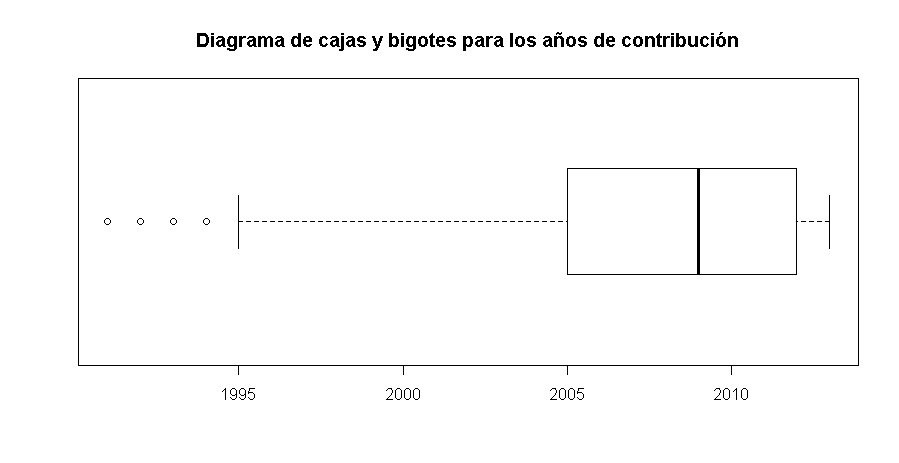
\includegraphics[scale=0.6]{density_year.png}
\caption{Diagrama de cajas y bigotes para los años en que se realizaron contribuciones}
\label{fig:figure-01}
\end{figure}

\begin{figure}[h!]
\centering
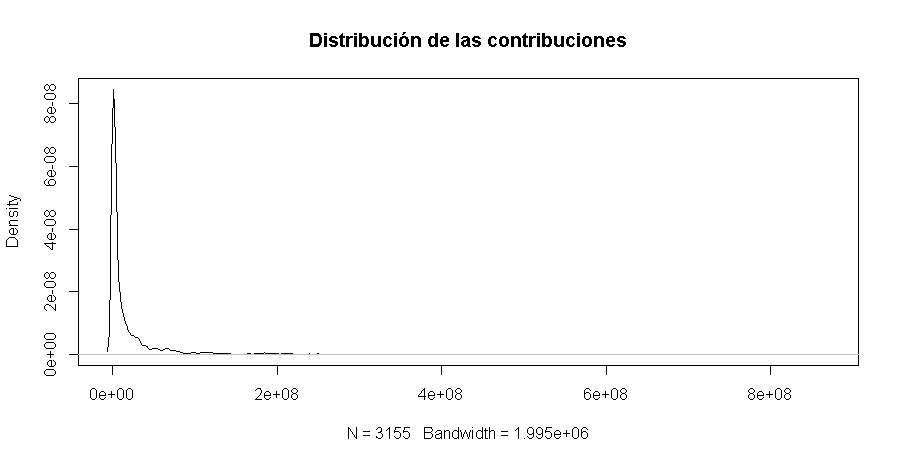
\includegraphics[scale=0.6]{density_amount2.png}
\caption{Distribución de las contribuciones}
\label{fig:figure-02} 
\end{figure}

\section{Conclusiones}
El análisis llevado a cabo hasta el momento puede extenderse para comprender las dinámicas de la geopolítica multilateral desde una perspectiva más objetivo. No obstante, dada la naturaleza de los datos, parece más conveniente optar por un análisis de serie de tiempo. Por otro lado, cabe destacar la presencia de varias variables categóricas en el conjunto de datos. Por consiguiente, es necesario extender el análisis hacia técnicas estadísticas que contemplen esta configuración particular de la muestra.

\begin{thebibliography}{9}

\bibitem{worldbankkaggle} 
World Bank Group. (Enero de 2018). \textit{Contributions to Financial Intermediary Funds}, Versión 297. Recuperado el 4 de abril de 2021 de {\tt https://www.kaggle.com/theworldbank/contributions-\\to-financial-intermediary-funds}.
\end{thebibliography}
	
\end{document}